\chapter{Multigrid solvers}\label{ch:multigrid}
\chapterstatus{written}{2026-11-17}

Screened modified-gravity theories have nonlinear elliptic field equations that cannot be solved with FFTs. \fml{} has a
general nonlinear multigrid solver on uniform, MPI-distributed grids in any dimension, with the field equations of
$f(R)$, DGP (and through it the cubic Galileon and Horndeski tables), the symmetron and the dilaton on top of it, and a
second solver on adaptively refined grids. In \file{SimulationCode} they give the exact fifth force
(\cref{sec:ext-quasistatic}, \cref{ch:mg-simulations}); they are also standalone tools for any nonlinear PDE.

\begin{modulebox}{MultigridSolver, AdaptiveMPIGrid}
\nsp{FML::SOLVERS::MULTIGRIDSOLVER}: \file{MultiGridSolver.h} (\cls{MultiGridSolver}, \cls{SolveResult}),
\file{FofrSolver.h} (\cls{FofrSolverCosmology}), \file{DGPSolver.h} (\cls{DGPSolverCosmology}), \file{SymmetronSolver.h},
\file{DilatonSolver.h}; the grids in \file{MPIGrid/MPIGrid.h} and \file{MPIGrid/MPIMultiGrid.h}.\par
\nsp{FML::SOLVERS::AMRMULTIGRIDSOLVER}: \file{AMRMultiGridSolver.h} (\cls{AMRMultiGridSolver}), \file{AMRDGPSolver.h}
(\cls{AMRDGPSolverCosmology}), \file{AMRSymmetronSolver.h}, \file{AMRDilatonSolver.h} (\cls{AMRDilatonSolverCosmology}); the grid in \file{AdaptiveMPIGrid/AdaptiveMPIGrid.h} (\cls{AdaptiveMPIGrid},
\cls{AdaptiveMPIGridTransfer}).\par
Documentation: \file{MultigridSolver/TerminationStatus.md}, \file{MultigridSolver/AMRMultiGridSolver.md},
\file{AdaptiveMPIGrid/README.md}. Examples: \file{MultigridSolver/examples} (Poisson, f(R), symmetron, DGP, AMR Poisson,
DGP and dilaton). Tests: \file{tests/test_multigrid.cpp}, \file{tests/test_multigrid_domain.cpp}, \file{AdaptiveMPIGrid/example}.
\end{modulebox}

\section{The full approximation scheme}\label{sec:mg-fas}

The equation is supplied as $L(f)=0$ in every cell, by a callback returning $L$ and $\partial L/\partial f_i$ (the
derivative with respect to the cell's own value, with the neighbours held fixed). The finest grid has $N^D$ cells
(level 0), each coarser level half as many per dimension, down to the coarsest the grid and its domain decomposition
allow. As the equation is nonlinear, the coarse levels carry the full solution, not only a correction: the full
approximation scheme (FAS) of Brandt \cite{Brandt1977,Trottenberg2001}.

\paragraph*{Relaxation.} Newton--Gauss--Seidel: every cell is updated as
\begin{equation}
f_i\to f_i-\frac{L_i(f)-S_i}{\partial L_i/\partial f_i},
\end{equation}
with $S$ the FAS source ($S=0$ on level 0). The cells are visited by colours: chess-board (sum of the coordinates mod 2)
by default, so the $2D$ nearest neighbours of a cell have the other colour, or with the \emph{cube ordering}
(\code{set_cube_ordering}) $2^D$ colours from the parity of each coordinate, so all $3^D-1$ surrounding cells have another
colour. Equations with mixed derivatives (DGP) need the cube ordering for the result not to depend on the number of
threads and tasks. The sweep visits only the cells of the current colour, row by row, and the boundaries are exchanged
after each colour. A custom pointwise update (\code{set_custom_update}) can replace the Newton step by an exact solve of the
local equation (used by $f(R)$ and the dilaton).

\paragraph*{The V-cycle.} With $\mathcal R$ the restriction (the average of the $2^D$ fine cells) and $\mathcal P$ the
prolongation (cell-centred $D$-linear interpolation: in each direction the fine cell gets weight $3/4$ from its coarse cell
and $1/4$ from the neighbour towards it):
\begin{enumerate}
\item relax on level $\ell$ and compute the residual $r_\ell=S_\ell-L_\ell(f_\ell)$;
\item restrict the solution and the residual and set the coarse source
      \begin{equation}
      S_{\ell+1}=L_{\ell+1}(\mathcal Rf_\ell)+\mathcal Rr_\ell ;
      \end{equation}
\item relax on level $\ell+1$ and recurse down to the coarsest level, where the sweeps are repeated until the residual is
      reduced by a factor 10 (or at most $50\times$ the number of coarse sweeps; with MPI the coarsest level has as many
      slices as tasks);
\item going up, correct $f_\ell\to f_\ell+\mathcal P\left(f_{\ell+1}-\mathcal Rf_\ell\right)$ and relax again.
\end{enumerate}
At a fixed point the coarse correction vanishes and $L_0(f_0)=0$. For equations that determine $f$ only up to a constant on a
periodic grid ($L(f+c)=L(f)$, e.g.\ Poisson or DGP), the discretised nonlinear source does not have exactly zero mean, so
there is no exact solution and the residual stalls; \code{set_subtract_mean_residual} instead solves $L(f)=\langle L\rangle$
on every level. An optional mask holds boundary cells fixed (non-periodic domains, compile flag \code{USE_MASK}).

\paragraph*{Parallelism.} The grids are \cls{MPIGrid}s with extra ghost slices (\code{n_extra_slices_left/right}), split in
slabs or, given a \cls{Domain}, in pencils (\cref{ch:parallelism}); all levels share the decomposition. Sweeps,
restriction and prolongation are OpenMP loops. The pencil decomposition allows a deeper hierarchy than slabs.

\paragraph*{Termination.} After the initial fine-grid sweeps and after every V-cycle the root-mean-square residual on level 0
is passed to the convergence criterion: \code{ConvergenceCriterionResidual} ($\mathrm{rms}(r)<\epsilon$) or
\code{ConvergenceCriterionError} (relative to the residual after the first sweeps), or any user function. The decision is
collective over the MPI tasks, and the budget of V-cycles is the minimum over tasks. \code{solve} returns a \cls{SolveResult}
with the status \code{Converged}, \code{MaxIterations} or \code{NonFinite} (a non-finite residual on any level, reported at
the next checkpoint and taking precedence), the final and initial residual and the number of V-cycles. Defaults: 10 sweeps
on the fine, coarse and first steps, $\epsilon=10^{-4}$, at most 1000 V-cycles.

\begin{cppcode}[A nonlinear equation with the generic solver]
#include <FML/MultigridSolver/MultiGridSolver.h>
using namespace FML::SOLVERS::MULTIGRIDSOLVER;
MultiGridSolver<3, double> g(N, -1, verbose, periodic, 1, 1);   // -1: as many levels as possible
g.set_epsilon(1e-7);
g.set_ngs_sweeps(3, 3, 20);                                     // fine, coarse, first
g.set_initial_guess(0.0);
MultiGridFunction<3, double> eq = [&](MultiGridSolver<3, double> * sol, int level, IndexInt i) {
    auto nb = sol->get_neighbor_gridindex(level, i);
    double lap  = sol->get_Laplacian(level, nb), dlap = sol->get_derivLaplacian(level, nb);
    double f    = sol->get_Field(level, i);
    return std::pair<double, double>{lap - lambda * f * f * f - source(level, i),
                                     dlap - 3 * lambda * f * f};        // {L, dL/df}
};
auto result = g.solve(eq, g.ConvergenceCriterionResidual);
if (not result.converged()) { /* MaxIterations or NonFinite */ }
\end{cppcode}

The helpers give the field, the $2D+1$ and $3^D$ neighbour indices, the cell position, the gradient and Laplacian and
their derivatives, the variable-coefficient operator $\nabla\cdot[b(f)\nabla f]$ and its derivative, and higher-order
finite differences $\partial_if$ and $\partial_i^2f$ to $\order{h^{2p}}$ for $p=1$--4.

\section{Model equations}\label{sec:mg-models}

The cosmological solvers take the density contrast $\delta$ on a grid in a box of size $B$ (coordinates $x\in[0,1)^3$) and
return a fifth-force potential $\Phi_F$ in the units of the code's Newtonian potential, $\Phi_{\rm GR}=a^2\Phi/(H_0B)^2$, so the
total force is $-\nabla(\Phi_{\rm GR}+\Phi_F)$ (\cref{ch:simulation-code}). They share the options: sweeps (defaults 10 on the
fine and coarse levels, 40 on the first step), $\epsilon=10^{-6}$, a \emph{relative} criterion (residual below $\epsilon$
times the rms of the linear source, which keeps the meaning of $\epsilon$ as the source amplitude grows by orders of
magnitude through a simulation), a warm start from the previous step's solution (\code{set_previous_solution}; for $f(R)$ rescaled to the
new background), and the number of V-cycles of the last solve. All assume a background with $\rho_m\propto a^{-3}$.

\paragraph*{Hu--Sawicki $f(R)$} \cite{HuSawicki2007}. With $\Phi_F=a^2|f_R|/[2(H_0B)^2]$ the quasi-static scalaron
equation in box units is
\begin{equation}
\nabla^2\Phi_F=\frac13\cdot\frac32\Om a\,\delta-\Pi(a)\left[\left(\frac{\bar\Phi_F}{\Phi_F}\right)^{1/(n+1)}-1\right],\qquad
\Pi=\frac{a^4}{2}\frac{R(a)c^2}{3H_0^2},
\end{equation}
with the background $R c^2/3H_0^2=\Om a^{-3}+4(1-\Om)$ (flat $\Lambda$CDM) or any $R(a)$ (\code{set_background_ricci}) and
$|\bar f_R|(a)=|f_{R0}|[R_0/R(a)]^{n+1}$. Two field variables (\param{gravity_model_fofr_multigrid_method}):
\begin{itemize}
\item \code{sqrt} (default): $\Phi_F=u^2$ \cite{Bose2017} with the standard Laplacian of $\Phi_F$. For $n=1$ the equation in
      a cell is a cubic $u^3+pu+q=0$ with $q<0$, which has exactly one positive root; the update solves it exactly (by a
      safeguarded Newton--bisection from the current value), so $\Phi_F>0$ on every level. For $n\ne1$ the local equation is
      strictly monotone in $u$ and is solved the same way. It converges for any $f_{R0}$, $n$ and redshift.
\item \code{log}: $\Phi_F=e^f$ with $\nabla\cdot(e^f\nabla f)$ \cite{Oyaizu2008,Li2012ECOSMOG}, the original method. The Newton
      steps can overshoot and give NaN far from the background, e.g.\ for $|f_{R0}|=10^{-6}$ at $a\lesssim0.5$.
\end{itemize}
The two discretise the kinetic term differently; the fifth forces agree to 0.1--0.5\% where both converge.

\paragraph*{Normal-branch DGP} \cite{Dvali2000,Schmidt2009,Li2013DGP}. In box units, with $\Phi_F=\phi/2$,
\begin{equation}
\nabla^2\phi+\frac1\alpha\left[(\nabla^2\phi)^2-(\nabla_i\nabla_j\phi)^2\right]=\frac{\Om a}{\beta}\delta,\qquad
\alpha=\frac{3\beta a^4}{(r_cH_0)^2}.
\end{equation}
The second derivatives use the $3^3$ surrounding cells, so the cube ordering is used, and $\phi$ is fixed only up to a
constant, so the mean residual is subtracted. The equation is solved for $\nabla^2\phi$ with the operator splitting
\cite{Li2013DGP}: with $w=1/3$ and $\Sigma=(\nabla_i\nabla_j\phi)^2+\alpha\Om a\delta/\beta-w(\nabla^2\phi)^2$,
\begin{equation}
L=\nabla^2\phi-\frac{\alpha}{2(1-w)}\left[\sqrt{1+\frac{4(1-w)\Sigma}{\alpha^2}}-1\right],\qquad
\frac{\partial L}{\partial\phi_i}=-\frac{6}{h^2}.
\end{equation}
In 3D the choice $w=1/3$ makes the derivative of the square root with respect to the centre cell vanish, so the Laplacian's
Jacobian is exact (the class throws for $D\ne3$). For $\delta\ge-1$ the discriminant is $\ge1/9$ for DGP; a negative value means a
bad density field and stops the solver. The cubic Galileon and Horndeski tables use the same equation with their $r_c(a)$
and $\beta(a)$; the cubic Galileon has no real solution in deep voids \cite{Barreira2013}, where
\code{set_allow_negative_discriminant} sets the discriminant to zero and counts the cells.

\paragraph*{Symmetron} \cite{HinterbichlerKhoury2010,Brax2012}, generalised to the powers $(N,M)$ of the potential (even
integers $M>N\ge2$; $(2,4)$ is the original). With $\chi=\phi/\phi_*$ and $\xi=H_0L_C/c$ ($L_C$ the vacuum Compton
wavelength),
\begin{equation}
\nabla^2\chi=\frac{a^2(H_0B)^2}{(M-N)\xi^2}\left[\chi^{N-1}\left(\left(\frac{a_{\rm ssb}}{a}\right)^3(1+\delta)-1\right)+\chi^{M-1}\right],
\end{equation}
with the background $\bar\chi=[1-(a_{\rm ssb}/a)^3]^{1/(M-N)}$ (zero before symmetry breaking) and
$\Phi_F=\frac{3(M-N)}{N}\Om a^2\beta^2(\xi/H_0B)^2a_{\rm ssb}^{-3}\,\chi^N$.

\paragraph*{Dilaton} \cite{Brax2012}. With $A(\phi)=1+A_2\phi^2/2M_{\rm pl}^2$, $m(a)=m_0a^{-r}$, $\xi=H_0/m_0$,
$s=9\Om A_2\xi^2$, $p=2r-3$ and $w=\phi/\bar\phi(a)=e^u$,
\begin{equation}
\nabla^2w=3A_2\Om a^2(H_0B)^2\,w\left[(1+\delta)a^{-3}-T(u)\right],\qquad T=(1+py)^{-3/p},\quad y=\frac{a^p-1}{p}+\frac us,
\end{equation}
where $T\to e^{-3y}$ for $p\to0$. The equation does not depend on $\beta_0$, and the fifth-force potential is
\begin{equation}
\Phi_F=\frac{a^2\beta(a)^2w^2}{2A_2(H_0B)^2},\qquad\beta(a)=\beta_0\exp\left[\frac{s(a^p-1)}{p}\right].
\end{equation} The multigrid works with $w$ and the standard Laplacian (so the coarse corrections are
averages of $\phi$) while the pointwise update solves for $u=\ln w$, where the local equation is strictly decreasing: the field
spans many orders of magnitude at early times ($u\sim\pm40$ in empty and full cells of a particle lattice at $z=30$), for
which the $\nabla\cdot(e^u\nabla u)$ form of the paper does not converge.

\begin{cppcode}[The exact f(R) fifth force]
#include <FML/MultigridSolver/FofrSolver.h>
FofrSolverCosmology<3> fofr(OmegaM, /*n*/ 1.0, /*fR0*/ 1e-5, H0Box, verbose);
fofr.set_ngs_steps(3, 3, 20);
fofr.set_epsilon(1e-6);
fofr.set_relative_criterion(true);
fofr.set_previous_solution(phiF_previous, a_previous);   // warm start (optional)
fofr.solve(a, delta_real, phiF_real);                     // FFTWGrid in, FFTWGrid out
\end{cppcode}

In \file{SimulationCode} the exact solvers are switched on with \code{gravity_model_<model>_exact_solution} and controlled
by \param{multigrid_nsweeps} (3), \param{multigrid_nsweeps_first_step} (20), \param{multigrid_solver_residual_convergence}
($10^{-6}$), \param{multigrid_convergence_criterion}, \param{multigrid_coarse_factor} (solve on a grid coarser than the force
grid, with the density restricted by \param{multigrid_coarse_restriction}) and \param{multigrid_start_redshift} with
\param{multigrid_force_before_start} (\cref{ch:mg-simulations}).

\begin{implementation}[Performance]
On a $128^3$ grid with a clustered COLA density, after removing the per-cell overheads (colour loops over only the cells of
a colour, strided neighbour indices, a Newton update for the $f(R)$ cubic instead of trigonometric roots) the exact $f(R)$ and
DGP forces cost about 40--50 times the GR PM force with 3 sweeps per level, and a whole COLA run 3.5--5 times the GR run; the
warm start saves about 20\% of the V-cycles. Fewer sweeps (2--3 instead of 10) are faster overall even though more V-cycles
are needed.
\end{implementation}

\section{Adaptive refinement}\label{sec:mg-amr}

To resolve screening inside halos beyond the uniform grid, \cls{AMRMultiGridSolver} solves the same kind of equations on an
adaptively refined grid, as in AMR codes for modified gravity \cite{Li2012ECOSMOG,Llinares2014,Puchwein2013} based on adaptive
meshes \cite{Kravtsov1997,Teyssier2002}.

\paragraph*{The grid.} \cls{AdaptiveMPIGrid} stores only the leaves of an octree on $[0,1)^D$ as a linear tree sorted along a
Peano--Hilbert curve \cite{Skilling2004}; each task owns a contiguous segment of the curve. Cells are found by containment:
the key of a point is binary-searched among the leaf ranges, so coarser, same-level and finer neighbours are found the same way.
\code{adapt} applies refine/coarsen flags with 2:1 balance across faces, edges and corners (iterated until no task changes);
\code{load_balance} repartitions the curve by a weight. One layer of ghost leaves is exchanged, overlapping communication with
the interior cells; irregular exchanges use the NBX algorithm \cite{Hoefler2010} above 64 tasks. The leaf set does not depend
on the number of tasks (checked with a global hash). In 3D the partition is also a \cls{PeanoHilbertDomain}, so particles can
follow the grid.

\paragraph*{The solver} is FAS multigrid with the multi-level adaptive technique \cite{Brandt1977}:
\begin{itemize}
\item the levels are the grid truncated at every refinement level (level 0 the full grid, level 1 every finest leaf replaced
      by its parent, \ldots, down to uniform grids coarser than the base grid, ending at 4 cells per dimension); values move
      between levels by volume-averaged restriction and gathering;
\item on each level only the finest cells are relaxed (red--black Newton--Gauss--Seidel); the FAS source
      $S_c=L_c(\mathcal Rf)+\mathcal R(S-L(f))$ carries the refinement into the coarse cells, so the fixed point solves the
      composite equation on the leaves, at a cost per V-cycle proportional to the number of leaves;
\item the correction is prolonged linearly (with its gradient) into children; a cell that exists on both levels gets
      the coarse value itself (the same as adding the correction, but without the cancellation that turns a value that
      changed by many orders of magnitude, as the dilaton in a halo, into exactly zero); the coarsest level is relaxed until its residual drops by $10^3$;
\item the Laplacian is flux-conservative and cell-centred: across a coarse/fine face the fine cell uses a ghost value at its
      own tangential position (coarse value plus the coarse gradient times the offset), and the coarse cell the sum of the
      fluxes through the fine sub-faces, so the volume integral of the Laplacian vanishes exactly on a periodic grid; mixed
      second derivatives (\code{get_hessian}) are derivatives of the gradient field, lagged within a sweep.
\end{itemize}
\cls{AMRDGPSolverCosmology} is the DGP solver on these grids, with the same equation, splitting, units and options as
\cls{DGPSolverCosmology}, input and output per local leaf. The symmetron solver on these grids is
\cls{AMRSymmetronSolverCosmology} (\file{AMRSymmetronSolver.h}), and the dilaton solver \cls{AMRDilatonSolverCosmology}
(\file{AMRDilatonSolver.h}): the parameters, the equation for $w=\phi/\bar\phi(a)$, the relative criterion and the potential
$\Phi_F=\bar\Phi_F(a)w^2$ of \cls{DilatonSolverCosmology} (\cref{sec:mg-models}), with the same cell update in $u=\ln w$
(\code{DilatonSolverCosmology::solve_cell_affine}, shared by both, installed with \code{set_custom_update}). The update needs a
positive sum over the neighbours, so the coarse/fine ghosts use the minmod-limited coarse gradient (\code{set_coarse_fine_limiter};
with the unlimited gradient a ghost next to a screened halo in an $N$-body run went negative and the solve stalled); both options are
off by default. \code{get_equation} and \code{get_update} give the equation and the update to a code with its own solver
(\file{AMRCode}, partial solves). A \emph{partial solve} (\code{solve(eq, min_level)}) treats only the leaves at levels
$\geq$ \code{min_level} (and the coarser cells made of them) as unknowns and the rest as Dirichlet values, with V-cycles
that touch only the unknowns; it is what the adaptive $N$-body code \file{AMRCode} uses at its fine sub-steps
(\cref{sec:sr-amr}). The face table, most of the solver's memory, stores 32-bit indices. Limitations: no OpenMP yet,
no helper for $\nabla\cdot(b(f)\nabla f)$ (needed for $f(R)$), every multigrid level between the base level and the
finest holds a copy of the base leaves, and the AMR solver is not used by \file{SimulationCode}.

\begin{cppcode}[Poisson on an adaptive grid]
#include <FML/MultigridSolver/AMRMultiGridSolver.h>
using namespace FML::SOLVERS::AMRMULTIGRIDSOLVER;
AMRMultiGridSolver<3> solver(grid);                // an AdaptiveMPIGrid after adapt / load_balance
int id = solver.add_external_field(delta);         // per local leaf, restricted to all levels
AMREquation<3> eq = [id](const AMRMultiGridSolver<3> & sol, int level, IndexInt i) {
    auto [lap, dlap] = sol.get_laplacian(level, i);
    return std::pair<double, double>{lap - sol.get_external_field(id, level, i), dlap};
};
auto result = solver.solve(eq);
auto force  = solver.get_solution_gradient();      // D phi per leaf
\end{cppcode}

\begin{figure}[htbp]
\centering
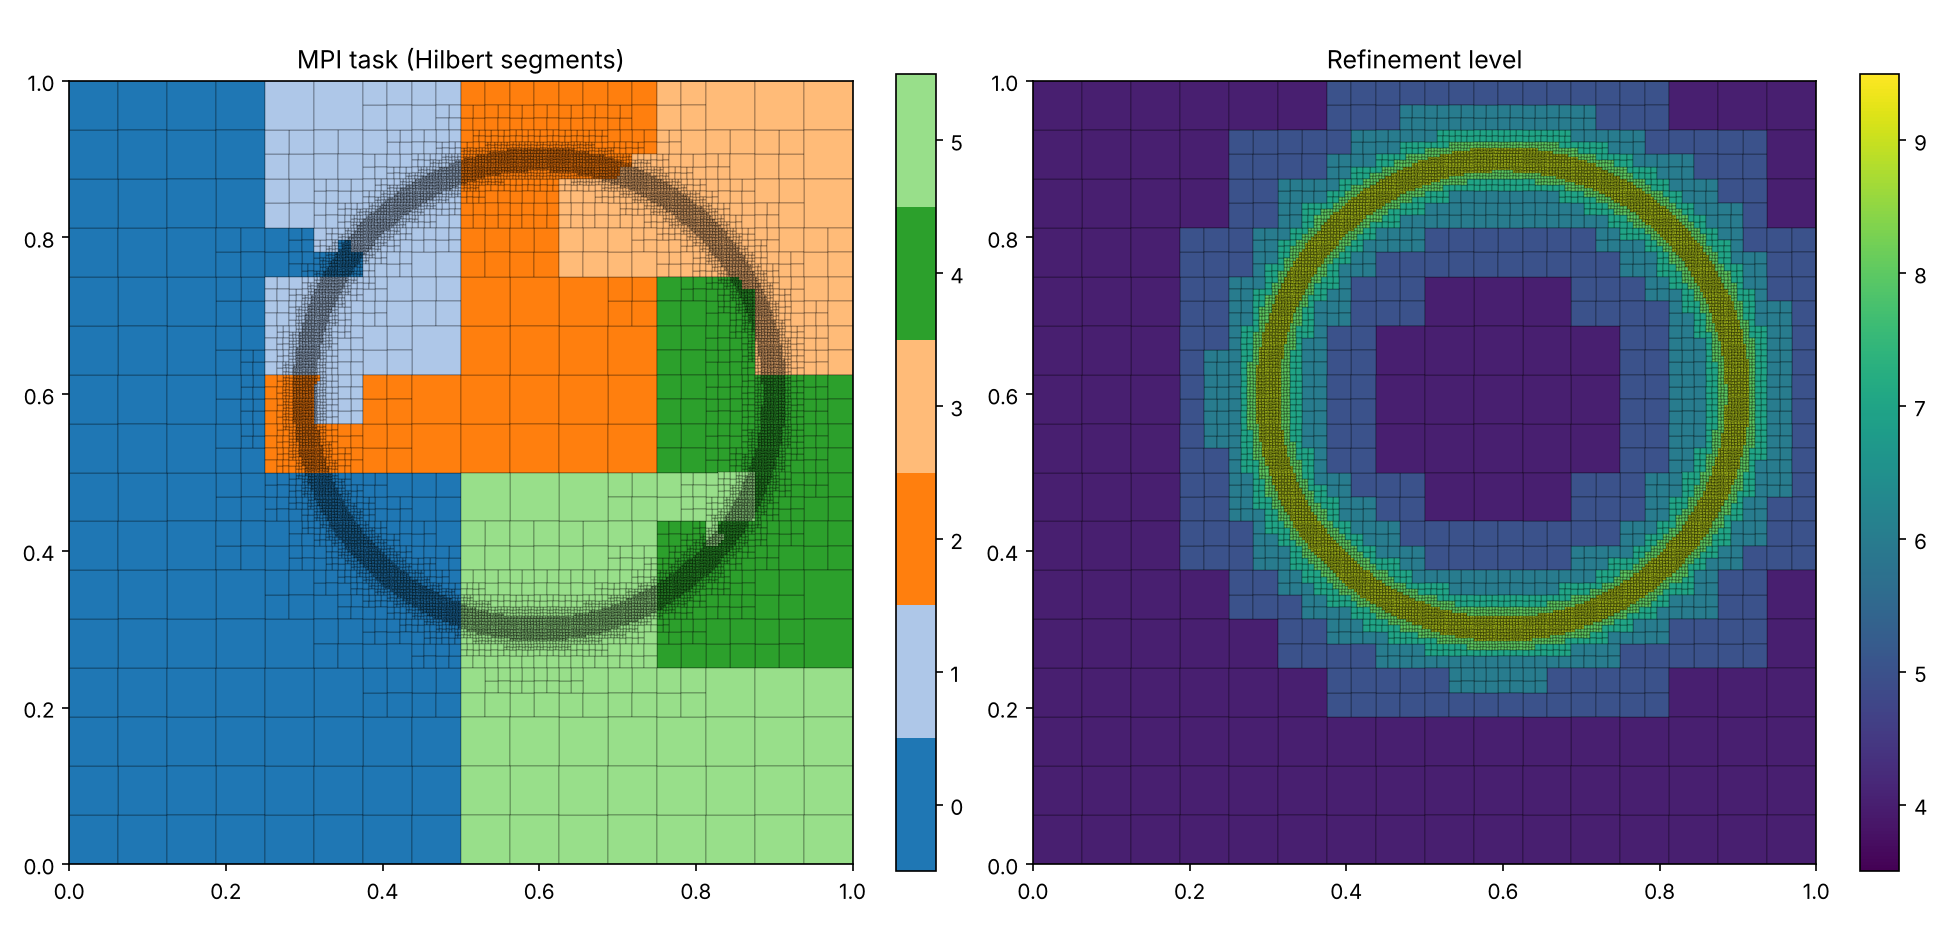
\includegraphics[width=0.9\textwidth]{amr_grid}
\caption{An \cls{AdaptiveMPIGrid} from its example (\file{AdaptiveMPIGrid/example}): a 2D grid refined around a ring from level 4 to level 9
with 2:1 balance, on 6 MPI tasks. \emph{Left:} the task owning each leaf, contiguous segments of the Peano--Hilbert curve.
\emph{Right:} the refinement level.}
\label{fig:mg-amr}
\end{figure}


\section{Validation}\label{sec:mg-validation}

\begin{validation}[Validation: uniform grids]
\file{tests/test_multigrid.cpp} on 1, 2 and 4 tasks: the finite-difference helpers against analytic derivatives (orders 1--4);
Poisson with a white-noise source reduces the residual by more than a factor 5 per V-cycle (2+2 sweeps); a DGP-type equation
with mixed derivatives converges with the cube ordering and the mean residual subtracted; the $f(R)$ cubic, equal fifth forces
from the \code{sqrt} and \code{log} methods, and convergence of \code{sqrt} for $|f_{R0}|=10^{-6}$ at $a=0.5$ (where \code{log}
gives NaN) and for $n=2$; the symmetron (zero field before symmetry breaking, linear theory for a small cosine perturbation,
screening in a halo, the generalised $(N,M)$); the dilaton (the effective-potential minimum for $r=1$ and $3/2$, linear theory,
the exact discrete solution of a strongly nonlinear sine profile of Brax et al.\ \cite{Brax2012}, screening, the warm start); DGP
with a clustered field; and every termination status. \file{tests/test_multigrid_domain.cpp}: the same solutions on slabs and on
every pencil layout, with the $2D+1$ and $3^D$ stencils and a fourth-order one.
\end{validation}

\begin{validation}[Validation: adaptive grids]
Poisson ($\nabla^2\phi=\delta$, periodic, Gaussian $\phi$) and $\nabla^2u-500u^3=s$ (Dirichlet), refined around the peak: in 2D
the rms error is $6.2\times10^{-5}$ and $6.7\times10^{-5}$ for AMR levels 4--8 against $6.1\times10^{-5}$ and
$6.9\times10^{-5}$ for the uniform level 8, and converges at second order; the residual drops by 0.12--0.21 per V-cycle. DGP for a
compensated spherical overdensity with an exact force: rms force error $2.6\times10^{-3}$ of the peak force for AMR levels 4--7
(second order, 2.35), identical on 1--4 tasks, and on a uniform $32^3$ grid equal to \cls{DGPSolverCosmology} to
$7\times10^{-11}$. Dilaton (\file{examples/AMRDilatonExample.cpp}): the same overdensity, $A_2=5\times10^5$, $\xi=10^{-3}$, screened in
the centre ($w=0.16$ for $r=1$), against a radial Newton solution: rms errors of $w$ and of the force (of the peak) $1.8\times10^{-3}$
and $1.1\times10^{-2}$ on the uniform level 6, $1.9\times10^{-3}$ and $1.2\times10^{-2}$ for AMR levels 4--6 (5\% of the leaves), $5\times10^{-4}$
and $3.6\times10^{-3}$ for levels 5--7 (order 1.93 and 1.75); on a uniform $32^3$ grid ($\ln w$ from $-0.03$ to 10.1) $\Phi_F$ equals
\cls{DilatonSolverCosmology} to $5\times10^{-14}$; a first solve from $w=1$ in a peak with $1+\delta=2\times10^4$ resolved one level
below the finest converges in 4 V-cycles. Solutions are independent of the number of tasks (1--13) and clean under AddressSanitizer.
\end{validation}

\begin{validation}[Exact against approximate screening]
In a standalone comparison (not a regression test) for $f(R)$ on a $256^3$ grid of a $64\Mpch$ GR snapshot, the screening approximation of \file{SimulationCode} agrees with the
exact fifth force to 1--3\% in cells below the critical potential for F5 at $z=0$ and to 0.2\% for F4, but over-screens once a
large fraction of the volume has $|\Phi_N|$ above it (F6, F5 at $z=1$). Solving on a grid twice coarser than the force grid
keeps the total force source within 1\% for $k<2.3\hMpc$ but loses the fifth force above the coarse Nyquist frequency
(\cref{ch:mg-simulations}).
\end{validation}

\begin{figure}[htbp]
\centering
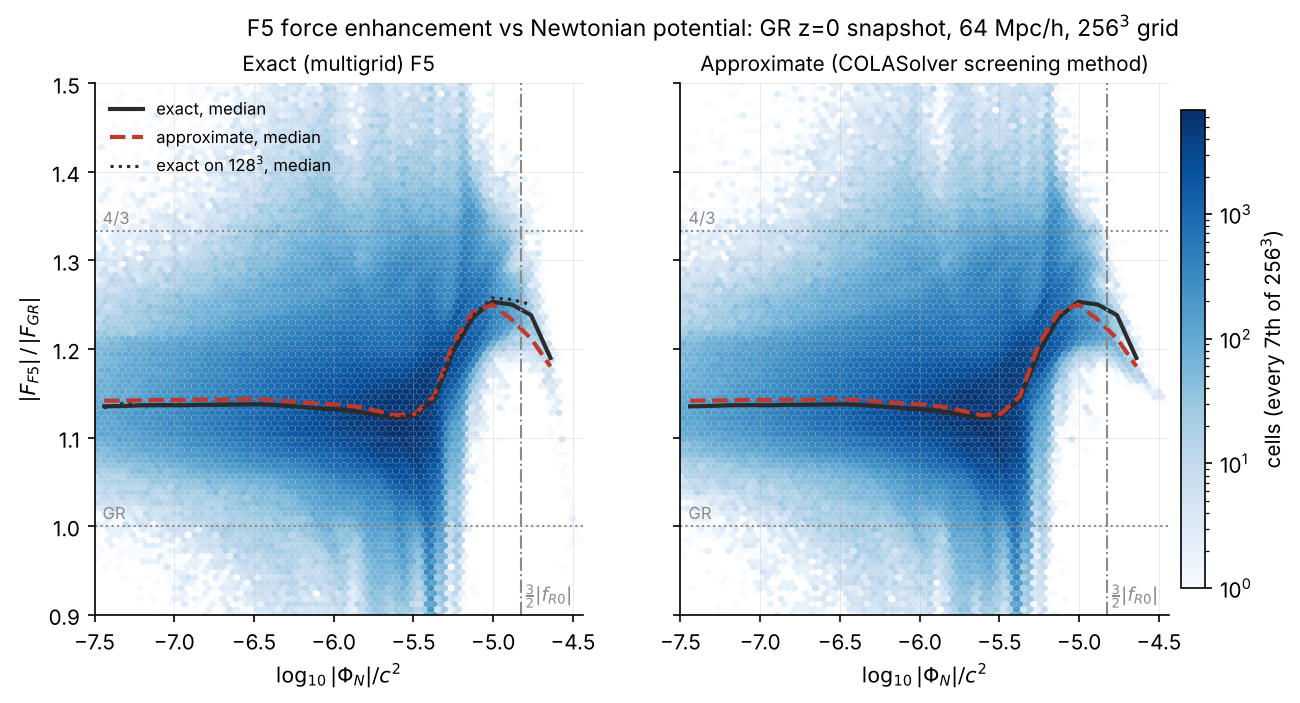
\includegraphics[width=\textwidth]{mg_f5_exact_vs_approx}
\caption{The F5 ($|f_{R0}|=10^{-5}$) force enhancement $|F_{F5}|/|F_{\rm GR}|$ against the Newtonian potential of the cell for a GR $z=0$
snapshot ($64\Mpch$, $256^3$ grid): the exact multigrid solution (\emph{left}) and the screening approximation of \file{SimulationCode}
(\emph{right}), with the medians of both (and of the exact solution on $128^3$). Unscreened cells have the linear enhancement
$\approx1.14$ at these scales (4/3 is the small-scale limit); screening sets in near $|\Phi_N|/c^2\sim\frac32|f_{R0}|$. A standalone
comparison, not a regression test.}
\label{fig:mg-f5}
\end{figure}

